% Условная компиляция для самостоятельной работы
\ifdefined\mainfile
    % Если это часть основного файла, не добавляем начало и конец документа
\else
    \documentclass[12pt, a4paper]{report}
    \usepackage{/Users/vladbelousov/Desktop/Semestr_4-FP-NSU/Настройка/library}
    \usepackage[utf8]{inputenc} % Подключение поддержки UTF-8
    \begin{document}
\fi

%%-------------------------------%%

\[ \begin{cases}
    x_2 =x_1  \\ 
    \displaystyle \theta_2 = \frac{n_1 \theta_1 }{n_2 } - \frac{x_1}{F_{12} } , \text{ где } \frac{1}{F_{12} } = \left( 1 - \frac{n_1}{n_2 }  \right)\frac{1}{R}    
\end{cases} \] 

Если выразить \( \theta_1  \) и \( \theta_2 \)  через \( z_1  \) и \(\displaystyle  z_2 \Rightarrow \frac{x_1}{\theta_1 } = -z_1 ,\text{ } \frac{x_1}{\theta_2 } = z_2    \), тогда получим из \( \displaystyle n_1 \left( \theta_1 +\frac{x_1}{R }\right) = n_2 \left( \theta_2 + \frac{x_1}{R }   \right)  \Rightarrow \)  

\[ n_1\left( - \frac{x_1}{z_1 } + \frac{x_1}{R }      \right) = n_2 \left( - \frac{x_1}{z_2 } + \frac{x_1}{R }   \right) \Rightarrow n_1\left( \frac{1}{z_1 } - \frac{1}{R }   \right) = n_2 \left( \frac{1}{z_2 } = \frac{1}{R }   \right) = \mathrm{inv}  \] 

Вывод: все лучи, выходящие из точки \( z_1 \), после преломления на сферической границе раздела 2-х сред пересекают ось \( z \) (или их продолжение) в точке \( z_2  \Rightarrow\)  гомоцентрический пучок после преломления остается гомоцентрическим.

Точки с координатами \( z_1 \) и \( z_2  \)  называются сопряженными.

1) Пусть \( z_1 \to  - \infty  \Rightarrow \) на границу падает слева параллельный пучок света: 

\[ \frac{1}{z_2 } = \left(  1 - \frac{n_1}{n_2 }  \right) \frac{1}{R } = \frac{1}{F_{12} } ;    \] 

\[ \text{ Если } (n_2 -n_1 )R >0: \] 

\begin{center}
    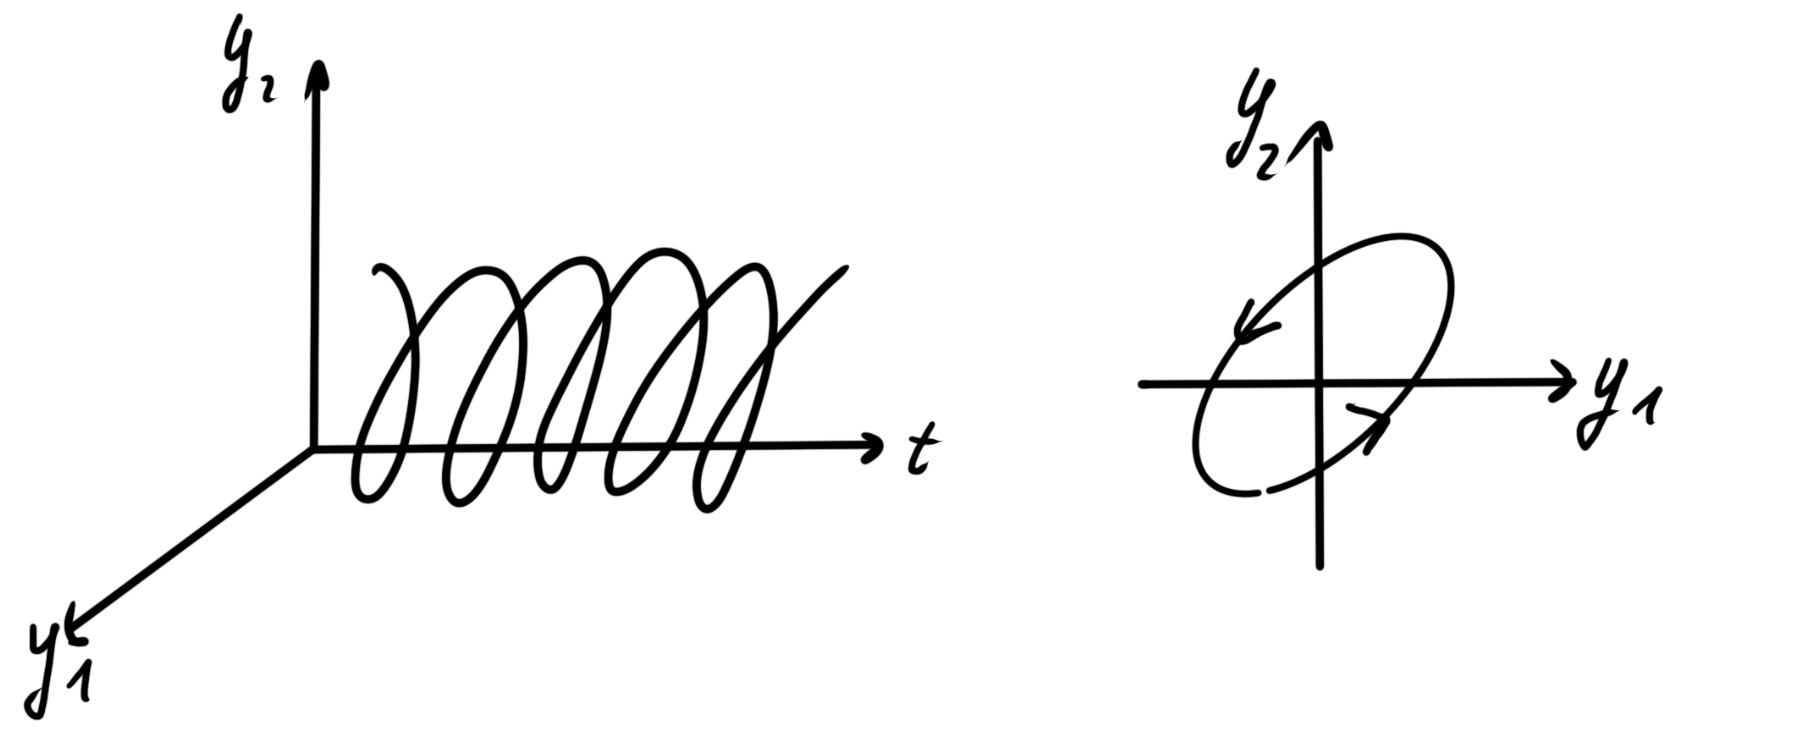
\includegraphics[width=0.5\textwidth]{/Users/vladbelousov/Desktop/Semestr_4-FP-NSU/ЭиО/Лекции_по_дням/image/71.png}
\end{center}

\[ \text{Если } (n_2 - n_1 )R <0:   \] 

\begin{center}
    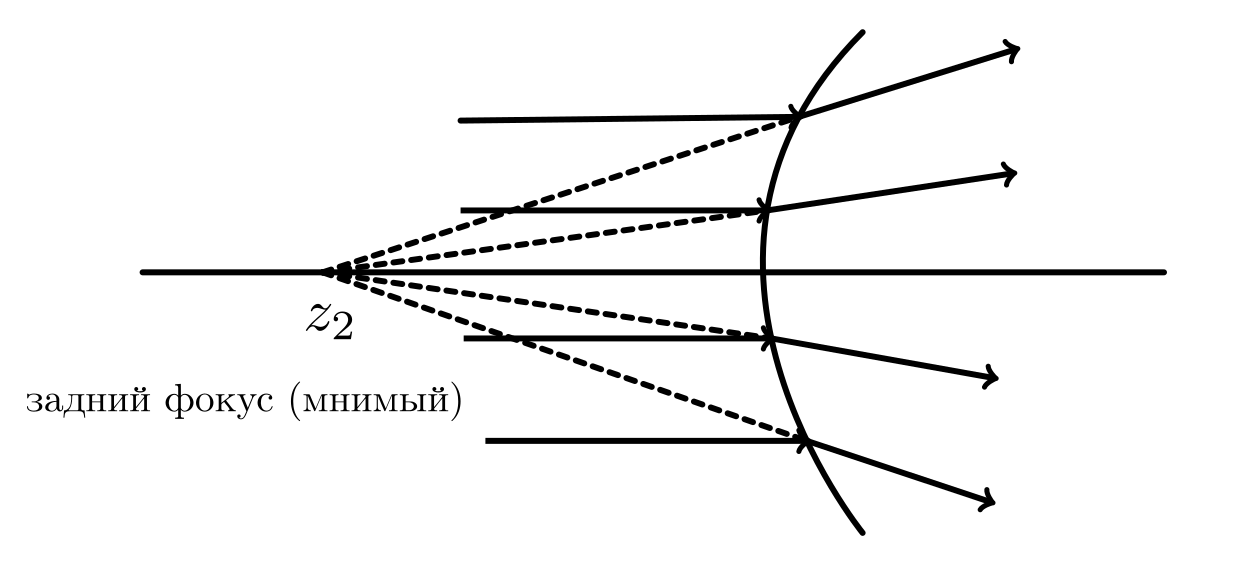
\includegraphics[width=0.5\textwidth]{/Users/vladbelousov/Desktop/Semestr_4-FP-NSU/ЭиО/Лекции_по_дням/image/72.png}
\end{center} 

2) Пусть \( z \to  \infty   \), после преломления параллельный пучок лучей \( \displaystyle  \frac{1}{z_1 } = \frac{1}{F_{12} } = \left( 1 - \frac{n_2}{n_1 }  \right) \frac{1}{R}    \) 

\[ \text{ Если } z_1>0 \Rightarrow (n_1 - n_2 )R >0 \] 

\begin{center}
    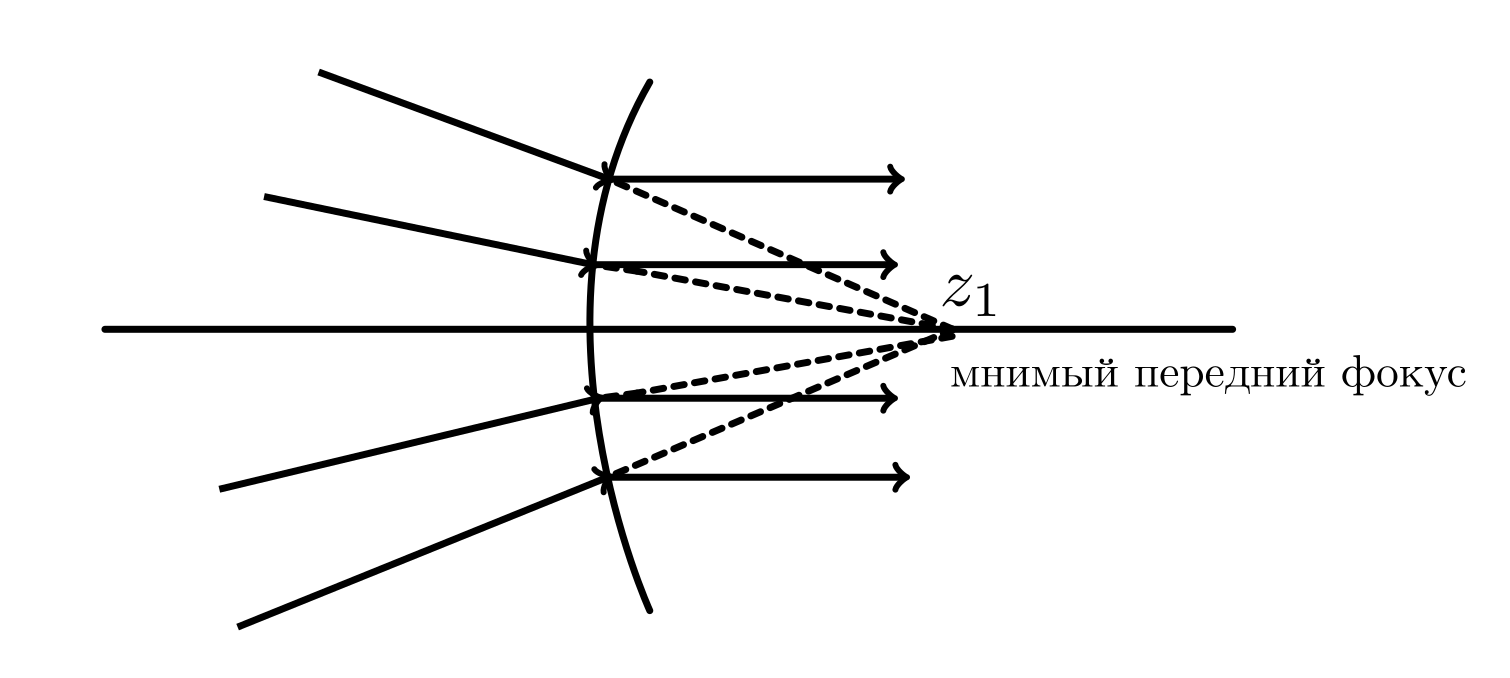
\includegraphics[width=0.5\textwidth]{/Users/vladbelousov/Desktop/Semestr_4-FP-NSU/ЭиО/Лекции_по_дням/image/73.png}
\end{center} 

\[ \text{ Если } z_1< 0 \Rightarrow (n_2 -n_1 )R < 0   \] 

\begin{center}
    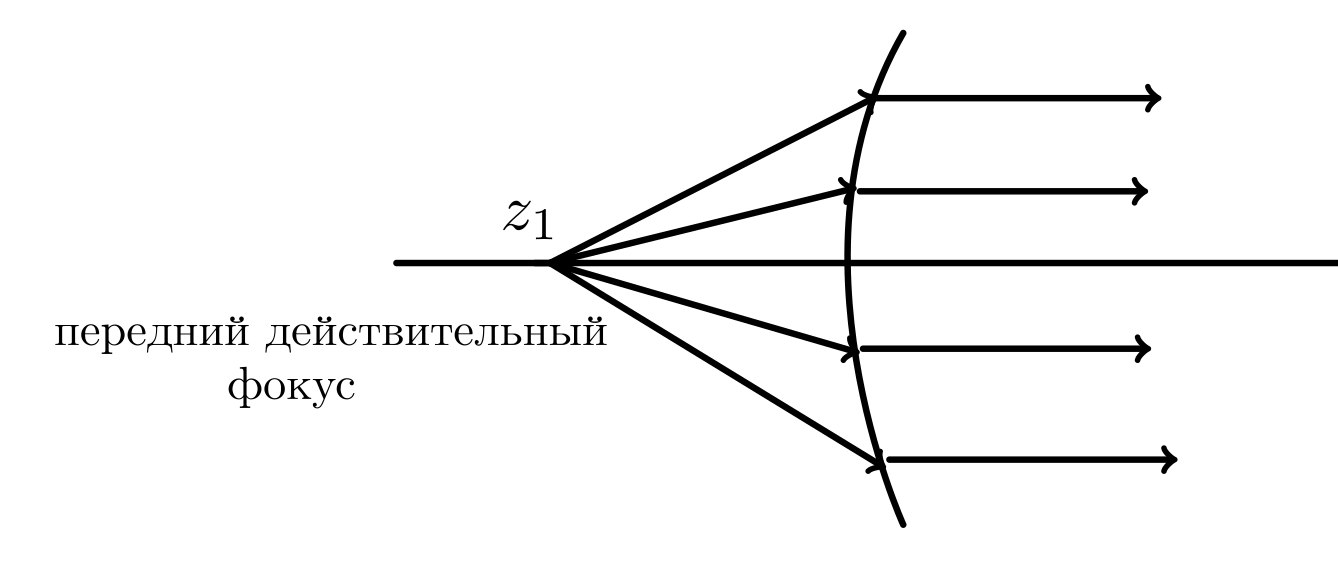
\includegraphics[width=0.5\textwidth]{/Users/vladbelousov/Desktop/Semestr_4-FP-NSU/ЭиО/Лекции_по_дням/image/74.png}
\end{center} 

\section{Матричный метод расчета центрированных оптических систем}

Матрица свободного пространства 

\begin{center}
    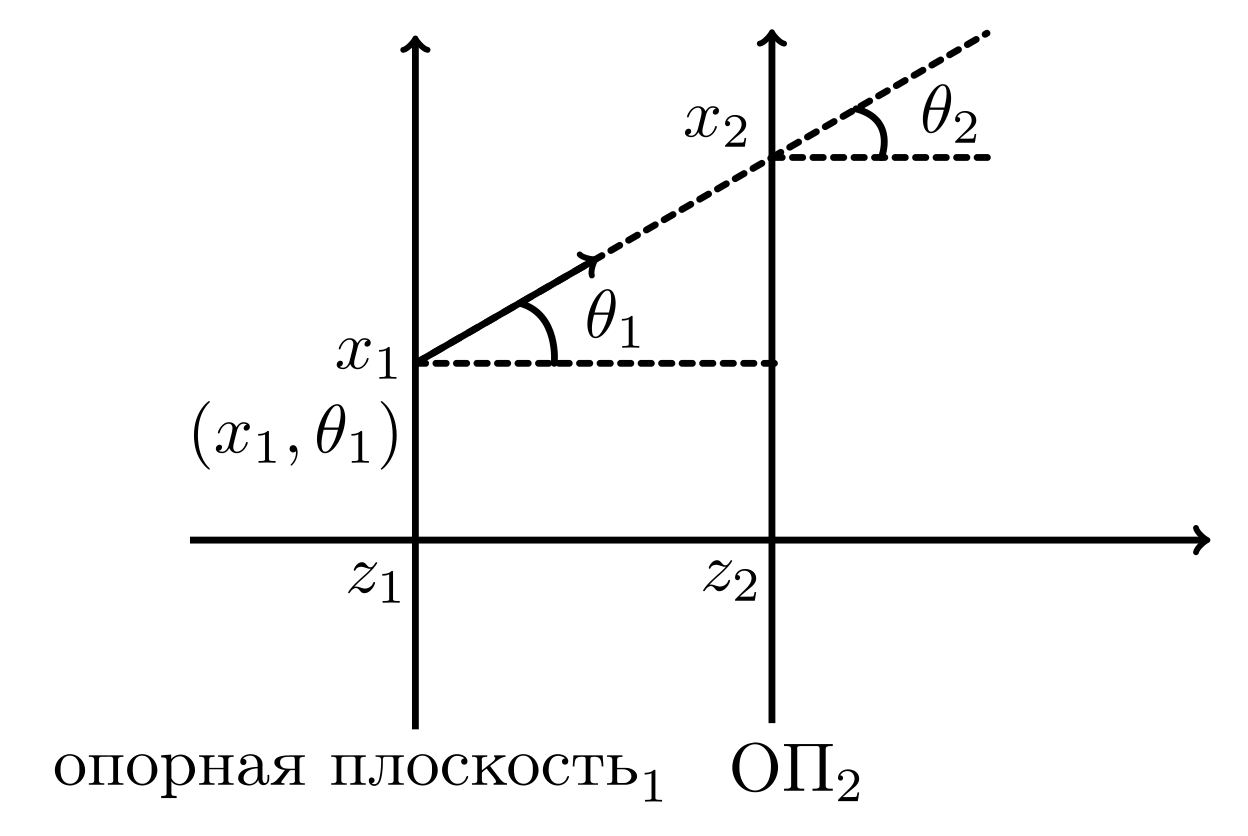
\includegraphics[width=0.5\textwidth]{/Users/vladbelousov/Desktop/Semestr_4-FP-NSU/ЭиО/Лекции_по_дням/image/75.png}
\end{center} 

\[ (x_1 , \theta_1 ) \text{ и  } (x_2 , \theta_2 )  \] 

\[ x_2 = x_1 + \theta_1 (z_2 -z_1 ) \Rightarrow x_2 = x_1 + x_1 ' (z_2 -z_1  ) \quad  (x_2 ' = x_1 ') \] 

\[ \theta \approx \mathrm{tg}   \theta = \frac{dx}{dz } = x ' \] 

\[ \frac{1}{F_{12} } = \left(  1 - \frac{n_1}{n_2 }  \right) \frac{1}{R}   \] 

Матрица перехода через границу раздела: 

\[ x_2 = x_1  , \text{ } \theta_2 = \frac{n_1 \theta_1 }{n_2 } - \frac{x_1}{F_{12} }  , \text{ } x_2 ' = \frac{n_1}{n_2 }x_1 ' -   \] 

\[ \begin{pmatrix}
x_2     \\
x_2 '
\end{pmatrix} = \begin{pmatrix}
1  & 0 \\
-\frac{1}{F_{12} }  & \frac{n_1}{n_2} 
\end{pmatrix} \begin{pmatrix}
x_1     \\
x_1' 
\end{pmatrix} \] 

Для удобства (чтобы матрица перехода имела \( \det =1 \)) вводят новые переменные: \( \displaystyle V_1 = n_1 x_1 ' , \text{ }  V_2 = n_2 x_2 '   \Rightarrow V_2 = V_1 - \frac{n_2 }{F_{12} } x_1  \):

\[ \begin{pmatrix}
x_2     \\
V_2
\end{pmatrix} = \begin{pmatrix}
1  & 0 \\
-\frac{n_2}{F_{12} }  & 1 
\end{pmatrix} \begin{pmatrix}
x_1     \\
V_1 
\end{pmatrix} \] 

При отражении луча от сферической границы

\begin{center}
    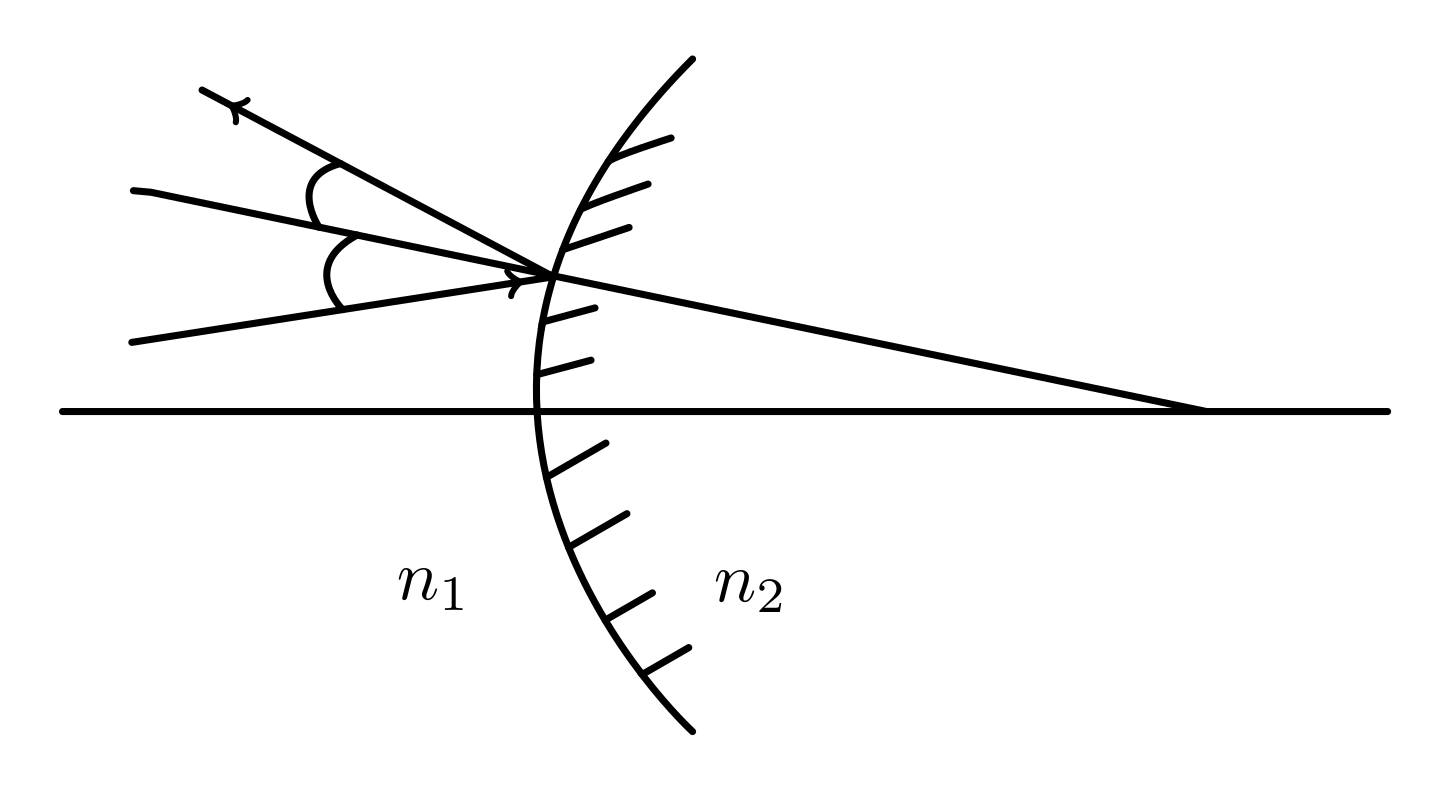
\includegraphics[width=0.5\textwidth]{/Users/vladbelousov/Desktop/Semestr_4-FP-NSU/ЭиО/Лекции_по_дням/image/76.png}
\end{center} 

Формулы предыдущие будут верны, если: \(n_2 = -n_1   \) 

Формула для матрицы свободного пространства отраженного луча: 

\[ \begin{pmatrix}
x_2     \\
V_2
\end{pmatrix} = \begin{pmatrix}
1  & \frac{z_2 - z_1 }{n }  \\
0  & 1 
\end{pmatrix} \begin{pmatrix}
x_1     \\
V_1 
\end{pmatrix} \]

\textbf{Матрица тонкой линзы (\(  \Delta x\) внутри линзы \( \ll x \))} 

\begin{center}
    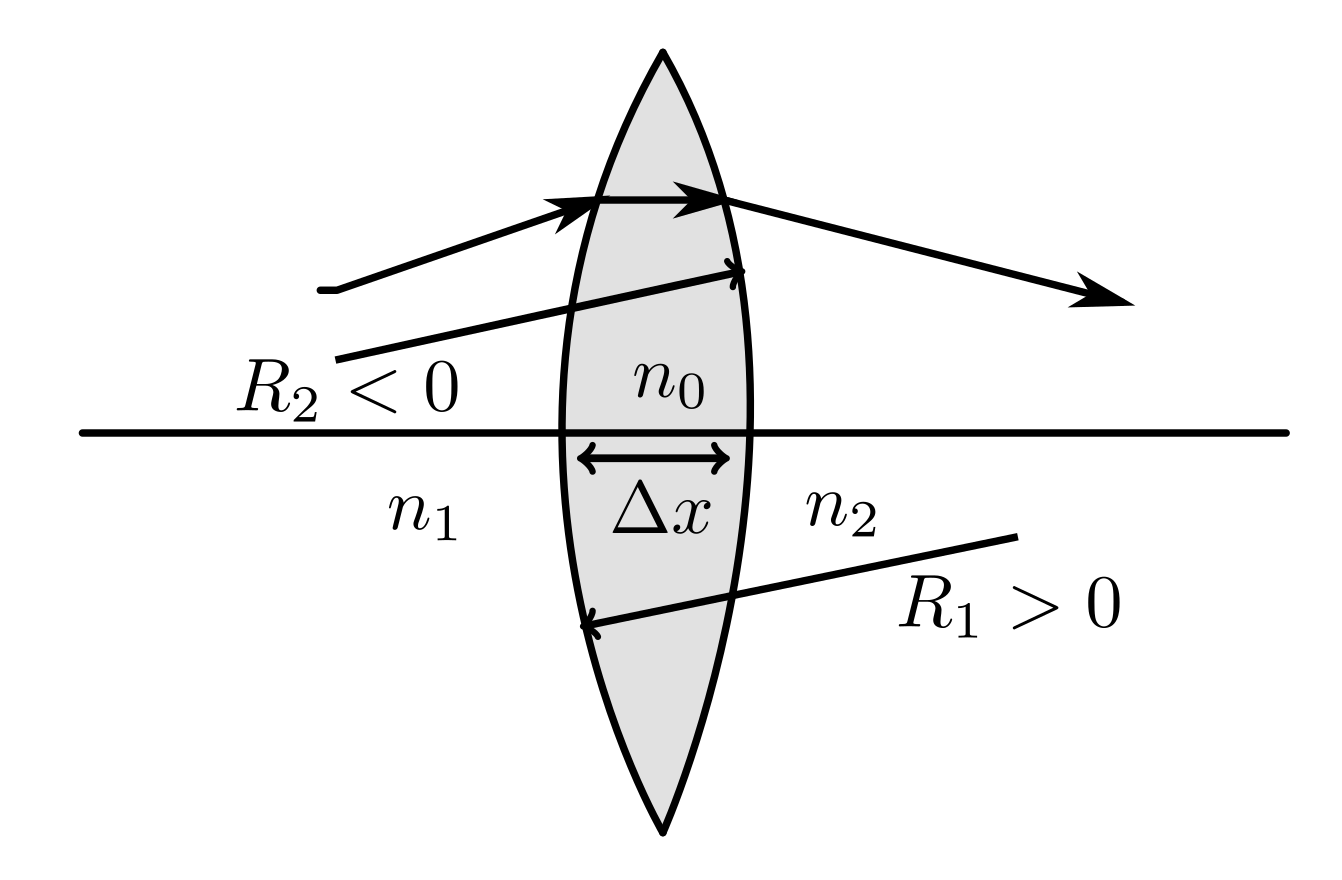
\includegraphics[width=0.5\textwidth]{/Users/vladbelousov/Desktop/Semestr_4-FP-NSU/ЭиО/Лекции_по_дням/image/77.png}
\end{center} 

\[ M= \begin{pmatrix}
    1  & 0  \\
    - \frac{n_2}{F_{02}}   & 1 
    \end{pmatrix}
    \begin{pmatrix}
        1  & 0  \\
        - \frac{n_0}{F_{10}}   & 1 
    \end{pmatrix} = \begin{pmatrix}
        1  & 0  \\
       - p    & 1 
\end{pmatrix} ; \text{ }  -p = - \frac{n_2}{F_{02} } - \frac{n_2}{F_{10}}   \] 
, где \( p  \) - оптическая сила.

Реальный случай \( n_1 = n_2 =1, \text{ } n_0 = n \) 

\[  p = (1 - n ) \frac{1}{R_2} + n \left( 1 - \frac{1}{n }  \right) \frac{1}{R_1} =   (n -1 ) \left(  \frac{1}{R_1 } - \frac{1}{R_2 }   \right) = \frac{1}{F_{\text{линзы} } }  \] 

\begin{center}
    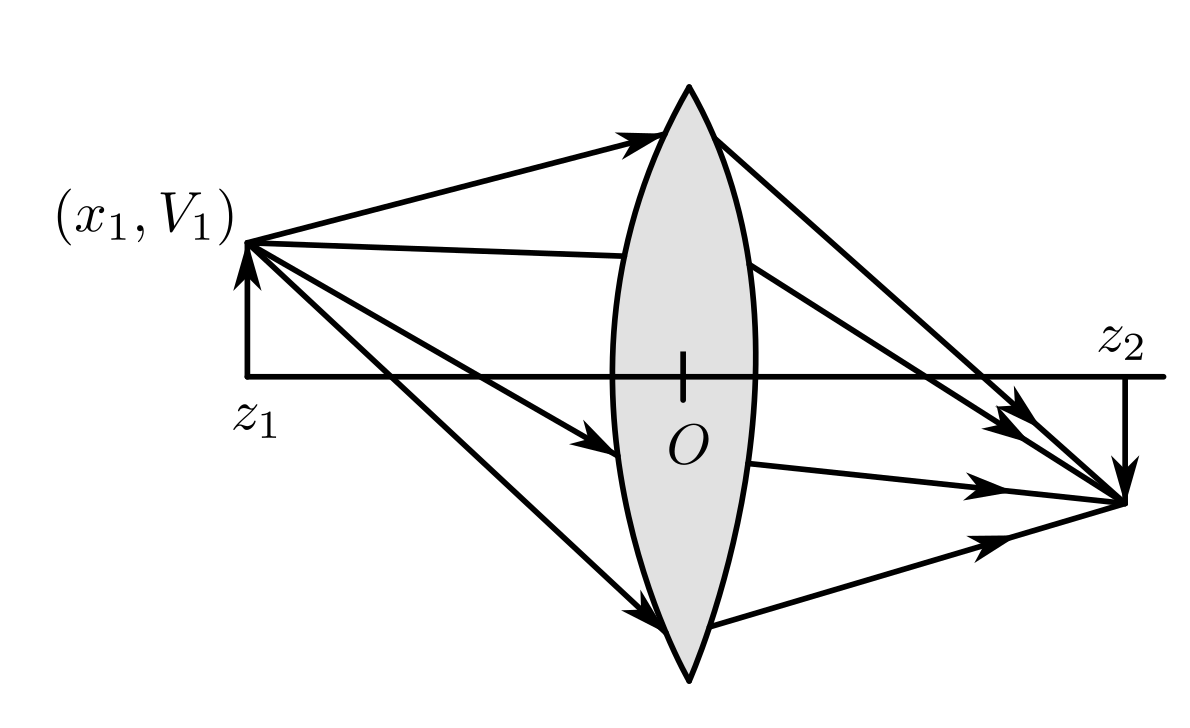
\includegraphics[width=0.5\textwidth]{/Users/vladbelousov/Desktop/Semestr_4-FP-NSU/ЭиО/Лекции_по_дням/image/78.png}
\end{center} 

\( x_2    \) и \( z_2 \) не зависят от \( V_1 \Rightarrow  \) точки \( (x_2 ,z_2 ) \) и \( (x_1 ,z_1 ) \) - сопряжение 

\[ \begin{pmatrix}
x_2 \\
V_2 
\end{pmatrix} =   
\begin{pmatrix}
    1  & z_2  \\
    0  & 1 
\end{pmatrix}
\begin{pmatrix}
    1  & 0  \\
    -\frac{1}{F}   & 1 
\end{pmatrix}
\begin{pmatrix}
    1  & z_1  \\
    0  & 1 
\end{pmatrix}
\begin{pmatrix}
    x_1 \\
    V_1
\end{pmatrix}
\] 

\[ \begin{pmatrix}
    x_2 \\
    V_2 
\end{pmatrix} =
\begin{pmatrix}
    1  & z_2  \\
    0  & 1 
\end{pmatrix}
\begin{pmatrix}
    1  & -z_1  \\
    0  & 1+\frac{z_1}{F}  
\end{pmatrix} 
\begin{pmatrix}
    x_1 \\
    V_1
\end{pmatrix}=
\begin{pmatrix}
    1- \frac{z_2}{F }   & -z_1 + z_2   \left( 1 + \frac{z_1}{F}  \right)\\
    - \frac{1}{F }  & 1+ \frac{z_1}{F}  
\end{pmatrix}
\begin{pmatrix}
    x_1 \\
    V_1
\end{pmatrix}
\] 

\[ x_2 = \left(  1 - \frac{z_2}{F }  \right) x_1 + \left(- z_1 + z_2 \left( 1 + \frac{z_1}{F }  \right) \right)V_1 , \text{ } x_2 \text{ в сопряжение не должен зависеть от } V_1   \] 


\[ \Rightarrow -z_1 + z_2 + \frac{z_1 z_2 }{F } = 0 \Rightarrow - \frac{1}{z_2 } + \frac{1}{z_1} + \frac{1}{F } = 0 \Rightarrow \frac{1}{z_1 } + \frac{1}{F } = \frac{1}{z_2 } \text{ }  (\text{формула тонкой линзы} )     \] 

\[\frac{x_2}{x_1 } = 1 - \frac{z_2}{F }  =\frac{z_2}{z_1}   \Rightarrow - 1 \frac{z_2}{ z_1 } + \frac{z_2}{F }  \Rightarrow \frac{z_2}{z_1 } = 1 - \frac{z_2}{F}    \] 

Если лучи идет параллельно оси \( z \), то \(\displaystyle  V_1  = 0:   \begin{pmatrix}
x_2\\
V_2 
\end{pmatrix}
\begin{pmatrix}
    1- \frac{z_2}{F }   & 0\\
    - \frac{1}{F }  & 1+ \frac{z_2}{F}  
\end{pmatrix}
\begin{pmatrix}
    x_1 \\
    0
\end{pmatrix}
\) 

\[ x_2 ' = V_2 = - \frac{x_1}{F }  \] 

\textbf{Матрица толстой линзы } 

\begin{center}
    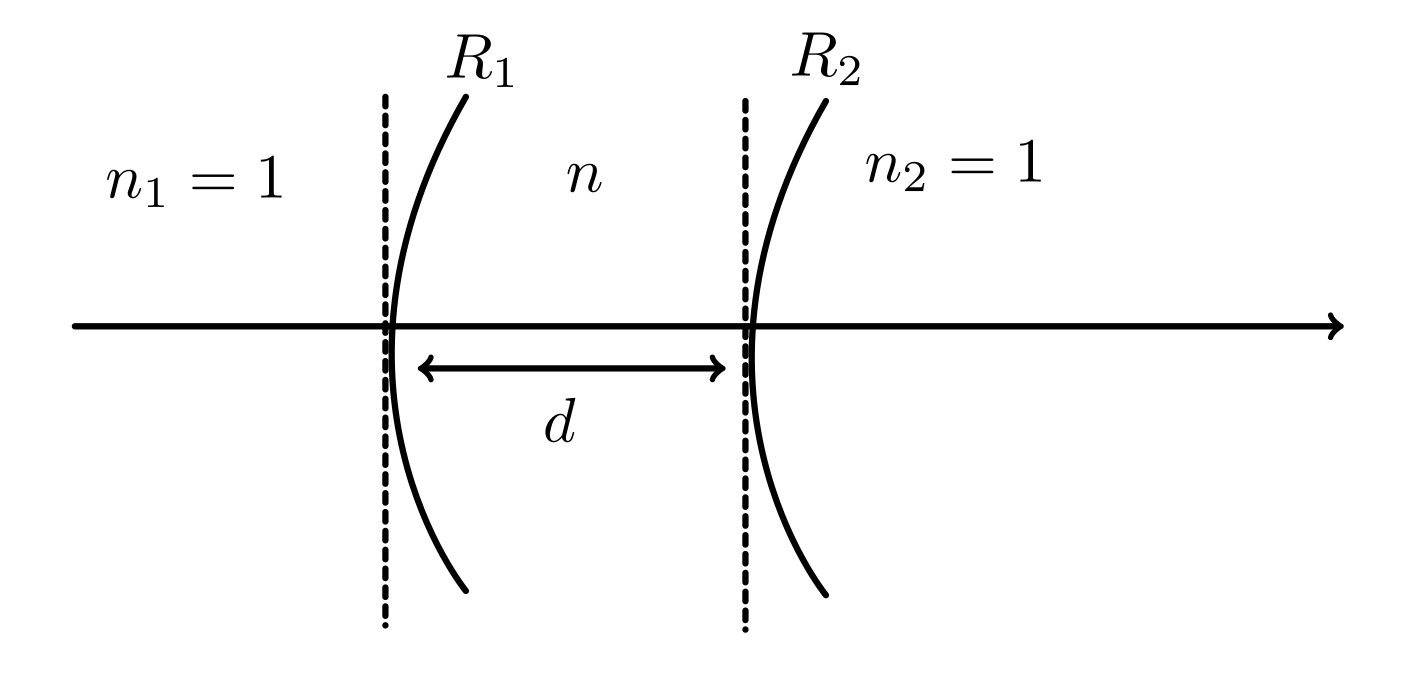
\includegraphics[width=0.5\textwidth]{/Users/vladbelousov/Desktop/Semestr_4-FP-NSU/ЭиО/Лекции_по_дням/image/79.png}
\end{center} 
\[ M = \begin{pmatrix}
    1  & 0\\
    - \frac{1}{F_{02} }  & 1
\end{pmatrix} 
\begin{pmatrix}
    1  & \frac{d}{n} \\
    0  & 1
\end{pmatrix}
\begin{pmatrix}
    1  & 0\\
    - \frac{n}{F_{10} }  & 1
\end{pmatrix}  = 
\begin{pmatrix}
    1  & 0\\
    - \frac{1}{F_{02} }  & 1
\end{pmatrix} 
\begin{pmatrix}
1 - \frac{d}{F_{10}}  & \frac{d}{n} \\
-\frac{n}{F_{02}}  & 1
\end{pmatrix}=
\begin{pmatrix}
    1 - \frac{d}{F_{10}}  & \frac{d}{n} \\
    - \frac{1}{F_0}   & 1- \frac{d}{n F_{02}} 
\end{pmatrix} 
\] 


\[ -\frac{1}{F_0 } = - \frac{1}{F_{02} }+ \frac{d}{F_{02} F_{10} } - \frac{n}{F_{10}}     \] 

\[ \frac{1}{F_0 } = (n -1 ) \left(  \frac{1}{R_1 } - \frac{1}{R_2 }    \right)  - d \frac{ 1 - n }{R_2 } \frac{1 - \frac{1}{n } }{R_1  } = (n -1 ) \left( \frac{1}{R_1 } - \frac{1}{R_2 }      \right) + \frac{d (n-1 ) ^2 }{n R_1 R_2 }     \] 

Пусть \( M = \begin{pmatrix}
m_{11}   & m_{12}\\
m_{21} & m_{22}
\end{pmatrix} \), как найти геометрически изображение источника 

\begin{center}
    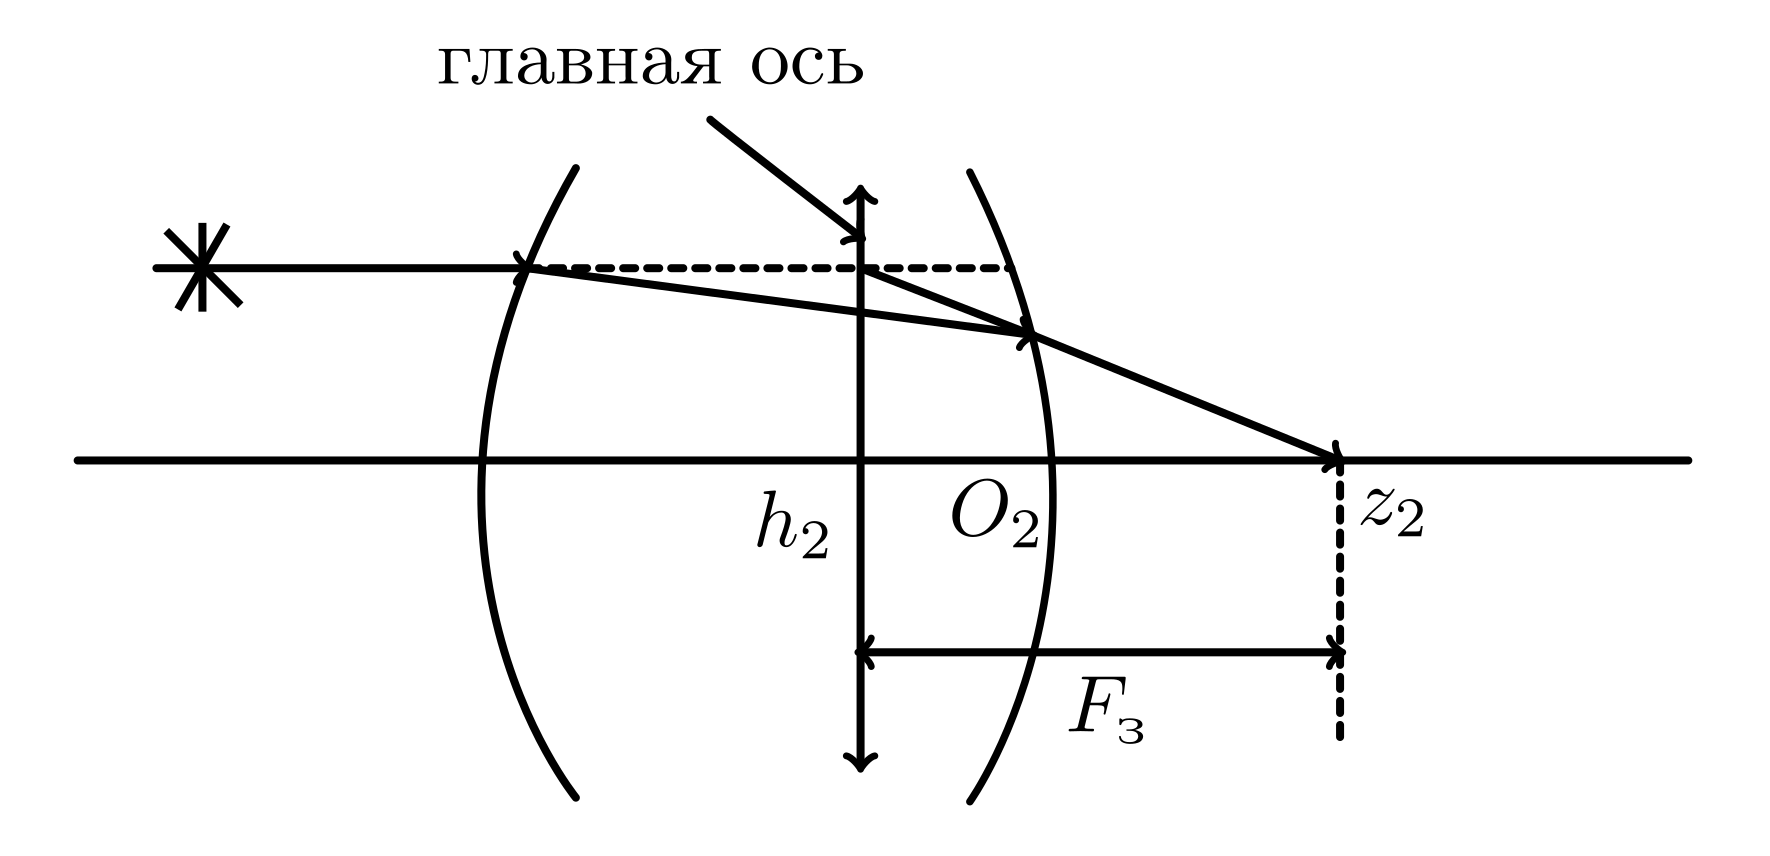
\includegraphics[width=0.5\textwidth]{/Users/vladbelousov/Desktop/Semestr_4-FP-NSU/ЭиО/Лекции_по_дням/image/80.png}
\end{center} 

\[ \begin{pmatrix}
    x_2\\
    V_2 
    \end{pmatrix}
    \begin{pmatrix}
        m_{11}   & m_{12}\\
        m_{21}  & m_{22}  
    \end{pmatrix}
    \begin{pmatrix}
        x_1 \\
        0
    \end{pmatrix}
\Rightarrow \begin{aligned}
x_2 &= m_{11} x_1 \\
V_2 &= x_2 ' = m_{21} x_1 
\end{aligned}    
\] 

\[ z_2 = \frac{x_2}{- x_2 ' } = \frac{m_{11} x_1 }{- m_{21} x_1 }= - \frac{m_{11}}{m_{21}}    \] 

\[ F_3 = \frac{x_1}{- x_2 ' } = \frac{x_1}{ - m_{21} x_1 } = - \frac{1}{m_{21}} = F_0 ,\text{ } h_2 = z_2 - F_3 = - \frac{m_{11}}{m_{21} } + \frac{1}{m_{21} } = \frac{1 - m_{11} }{m_{21}}       \] 

где \( h_2  \) - координата второй главной плоскости относительно точки \( O_2  \) 

\begin{center}
    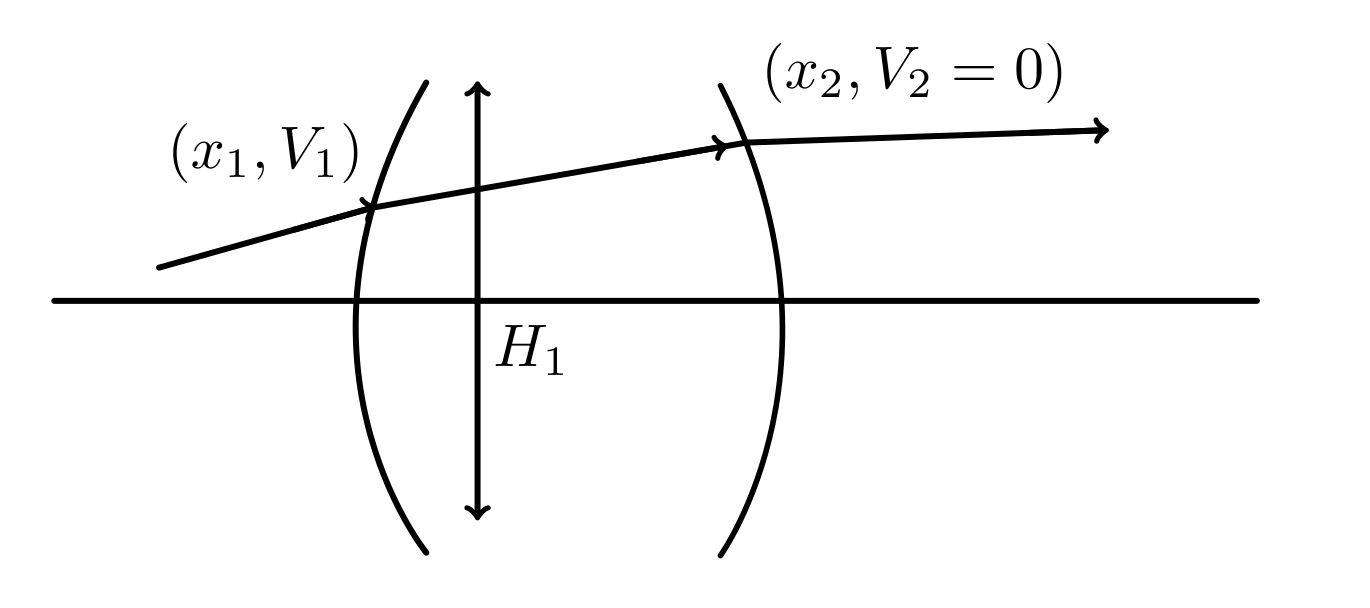
\includegraphics[width=0.5\textwidth]{/Users/vladbelousov/Desktop/Semestr_4-FP-NSU/ЭиО/Лекции_по_дням/image/81.png}
\end{center} 

\[ \begin{pmatrix}
x_1 \\
V_1 
\end{pmatrix} = M^{-1 }
\begin{pmatrix}
    x_2 \\
    0 
\end{pmatrix} =
\begin{pmatrix}
m_{22} & -m_{12}\\
-m_{21} & m_{11}
\end{pmatrix}\begin{pmatrix}
    x_2\\
    0 
\end{pmatrix}\] 

Способ построения: 

\begin{center}
    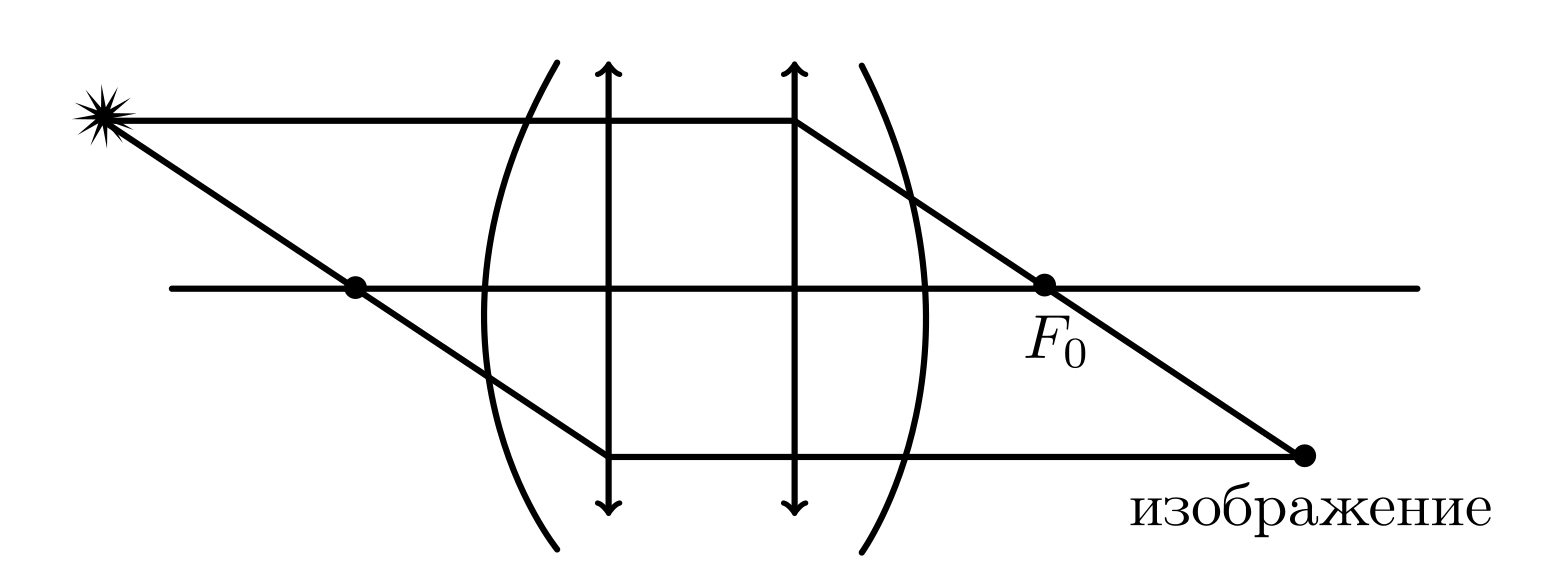
\includegraphics[width=0.5\textwidth]{/Users/vladbelousov/Desktop/Semestr_4-FP-NSU/ЭиО/Лекции_по_дням/image/82.png}
\end{center} 

%%-------------------------------%%

% Закрытие документа, если файл компилируется отдельно
\ifdefined\mainfile
    % Если это основной файл, не нужно заканчивать документ
\else
    \end{document}
\fi

